\chapter{Tracker}

We considerate tracker as an algorithm to detect a position of the object in
an image. We will present a few tested trackers and their results in this task.
Firstly we provide a short description of a simple straightforward tracker and
then we describe more complicated trackers.

We use the notion \emph{tracker} generally for an algorithm able to detect and
track an object (i.e. return an object position in the image).  We
differentiate between two types of tracker algorithms: \emph{detection based
algorithms} and \emph{sequence based algorithms}. Detection based algorithms
detect an object on each image separately. On the other hand, sequence-based
algorithms obtain, store and process information from a sequence of the past
images and use them for more accurate and faster tracking results. For this
task, we evaluate trackers in both categories.

%%%%%%%%%%%%%%%%%%%%%%%%%%%%%%%%%%%%%%%%%%%%%

\section {Detection based algorithms}
We denote as detection based algorithms all trackers, which detect an object on
Each image separately. These algorithms use only information obtained from
the current image and the information from the image on which the tracker was
initialized.

\subsection{Simple Background Tracker}

\emph{Simple Background Tracker} takes a photo of the background at the
beginning and we denote it as a \emph{pattern}. In order to detect an object in
a \emph{image}, a comparison of the \emph{image} and \emph{pattern} is taken.
We make this comparison by taking a sum of an absolute difference for each
color (Red, Green, Blue) in the images for each pixel.

As a result, we get a mask, where higher values mean the bigger difference between
the colors of the \emph{pattern} and \emph{image} at given pixel. We assume it
is caused by an object in front of the camera.  As the next step we will
binarize the mask with a given \emph{threshold}, \emph{blur} it and
\emph{threshold} again. At this point, we will find a contour with the biggest
area using OpenCV library. The center point of the rectangle of this contour
will be our estimation of the position of our object in the image. The whole
process is in the figure \ref{fig:simple-background-tracker}.

In the image is showed that between the photo of the background and the photo
of the object the light slightly changed (at the edge of the puzzle pieces). It
is causing noise, which we reduce by thresholding and blurring the image.

\begin{figure}
  \centering
  \begin{subfigure}[b]{0.48\linewidth}
    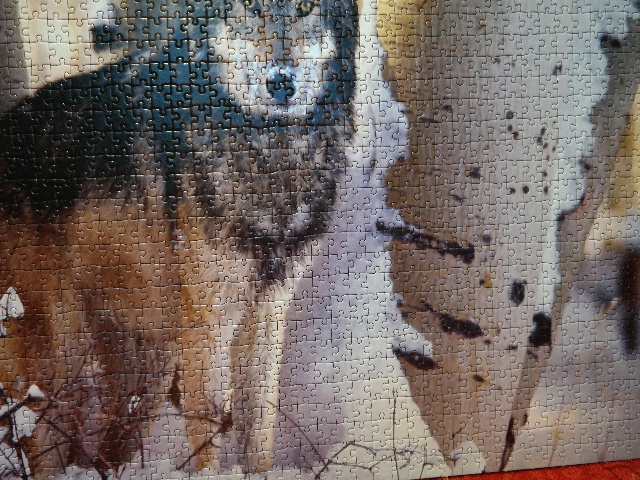
\includegraphics[width=\linewidth]{img/simple_background/background.jpg}
    \caption{Background}
  \end{subfigure}
  \begin{subfigure}[b]{0.48\linewidth}
    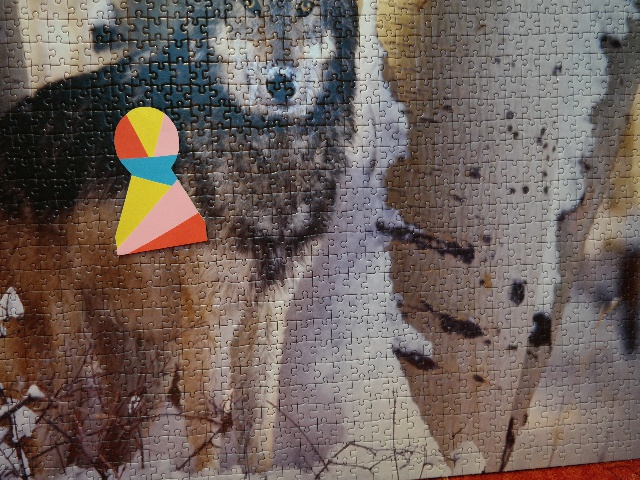
\includegraphics[width=\linewidth]{img/simple_background/object.jpg}
    \caption{Object}
  \end{subfigure}
  \begin{subfigure}[b]{0.48\linewidth}
    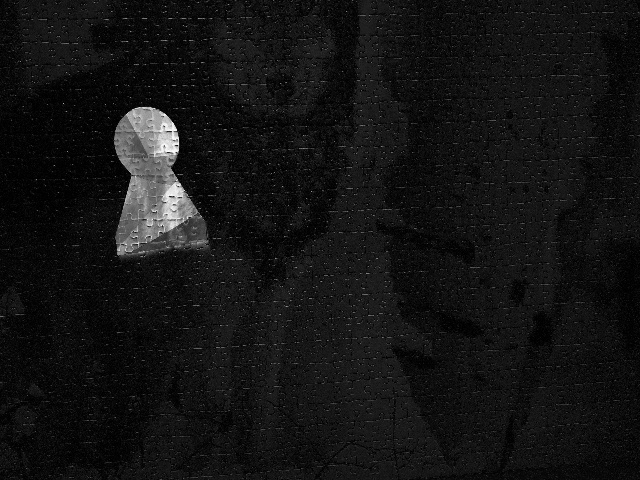
\includegraphics[width=\linewidth]{img/simple_background/rgb-diff.jpg}
    \caption{Sum of diffs in each channel (RGB)}
  \end{subfigure}
  \begin{subfigure}[b]{0.48\linewidth}
    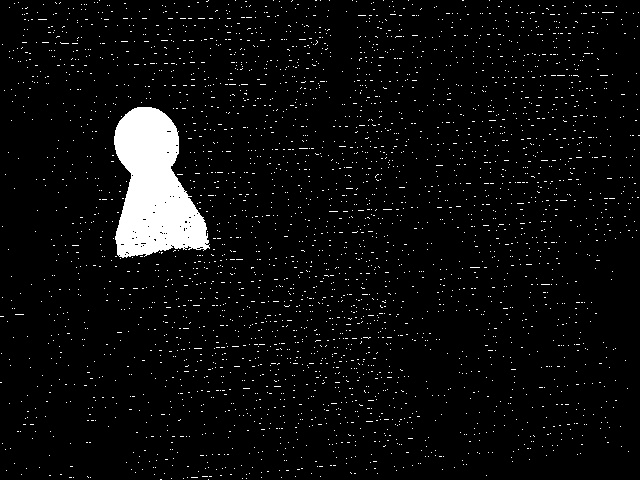
\includegraphics[width=\linewidth]{img/simple_background/first-thresh.jpg}
    \caption{Thresholded}
  \end{subfigure}
  \begin{subfigure}[b]{0.48\linewidth}
    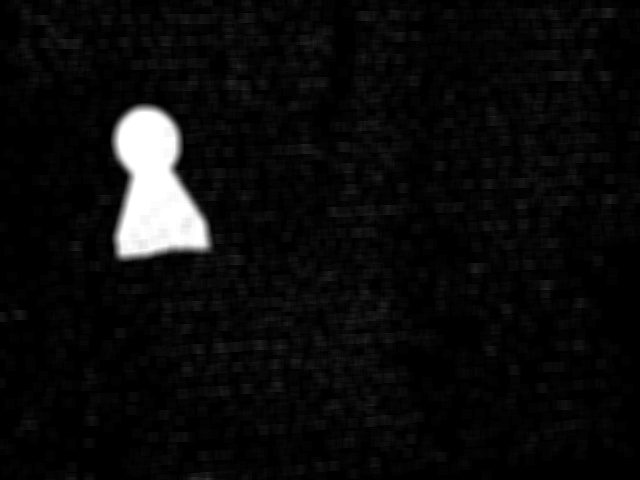
\includegraphics[width=\linewidth]{img/simple_background/blurring.jpg}
    \caption{Blurred}
  \end{subfigure}
  \begin{subfigure}[b]{0.48\linewidth}
    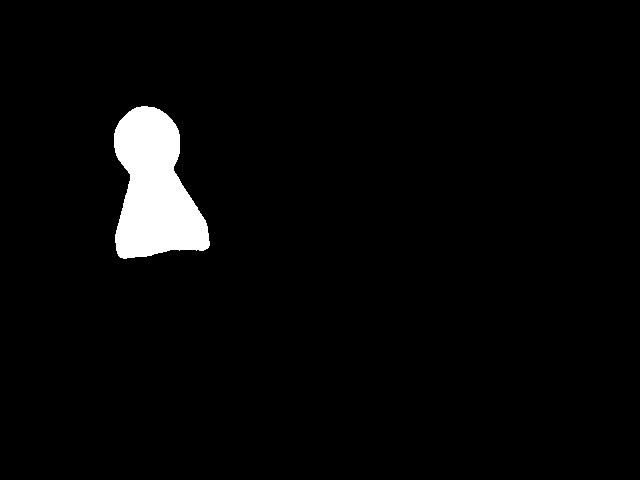
\includegraphics[width=\linewidth]{img/simple_background/second-thresh.jpg}
    \caption{Thresholded}
  \end{subfigure}
  \begin{subfigure}[b]{0.48\linewidth}
    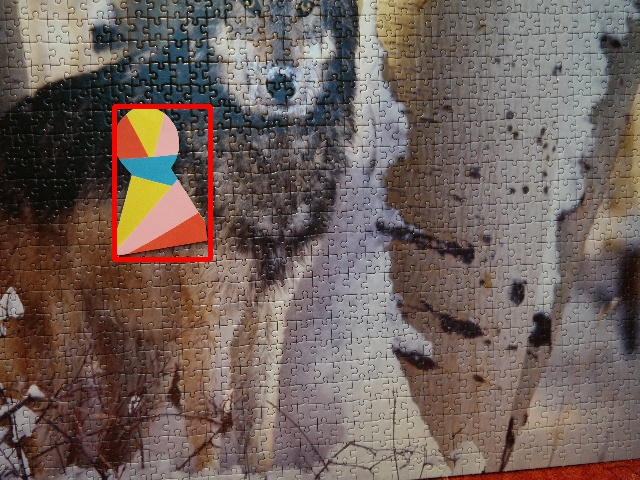
\includegraphics[width=\linewidth]{img/simple_background/result.jpg}
    \caption{Bounding box of the largest contour found.}
  \end{subfigure}
  \caption{Process of the simple background tracker}
  \label{fig:simple-background-tracker}
\end{figure}

As an advantage of this algorithm, we consider its simplicity and
straight-forward implementation. Furthermore, with a static background with
only one object moving it can reliably track an object without any information
about it.

On the contrary, it can not recover even from a little light changes or camera
movement. Also, an object moved by a human, for example, cannot be tracked
reliably, since the tracker recognizes the hand by the tracker as moving object
too.

\subsection{HSV tracker}

HSV tracker uses an idea of tracking an object by its color. Given an input
object described by a bounding box, we find the average color within the
bounding box. On a position request, we return a center of the largest area
with the color of the object.

We choose color coding via HSV (Hue, Saturation, Value). Unlike the RGB (Red,
Green, Blue) coding it can describe a color as Hue value, not triple values of
mixed colors. The approach of HSV color coding preserves one value -- hue
value,  even though the color is lighter or darker (like shadows in the image).
On the other hand in RGB coding shadows may cause a difference in all three
parts of coded color. Therefore an object description can be simplified
to one value.

\begin{figure}[h!]\centering
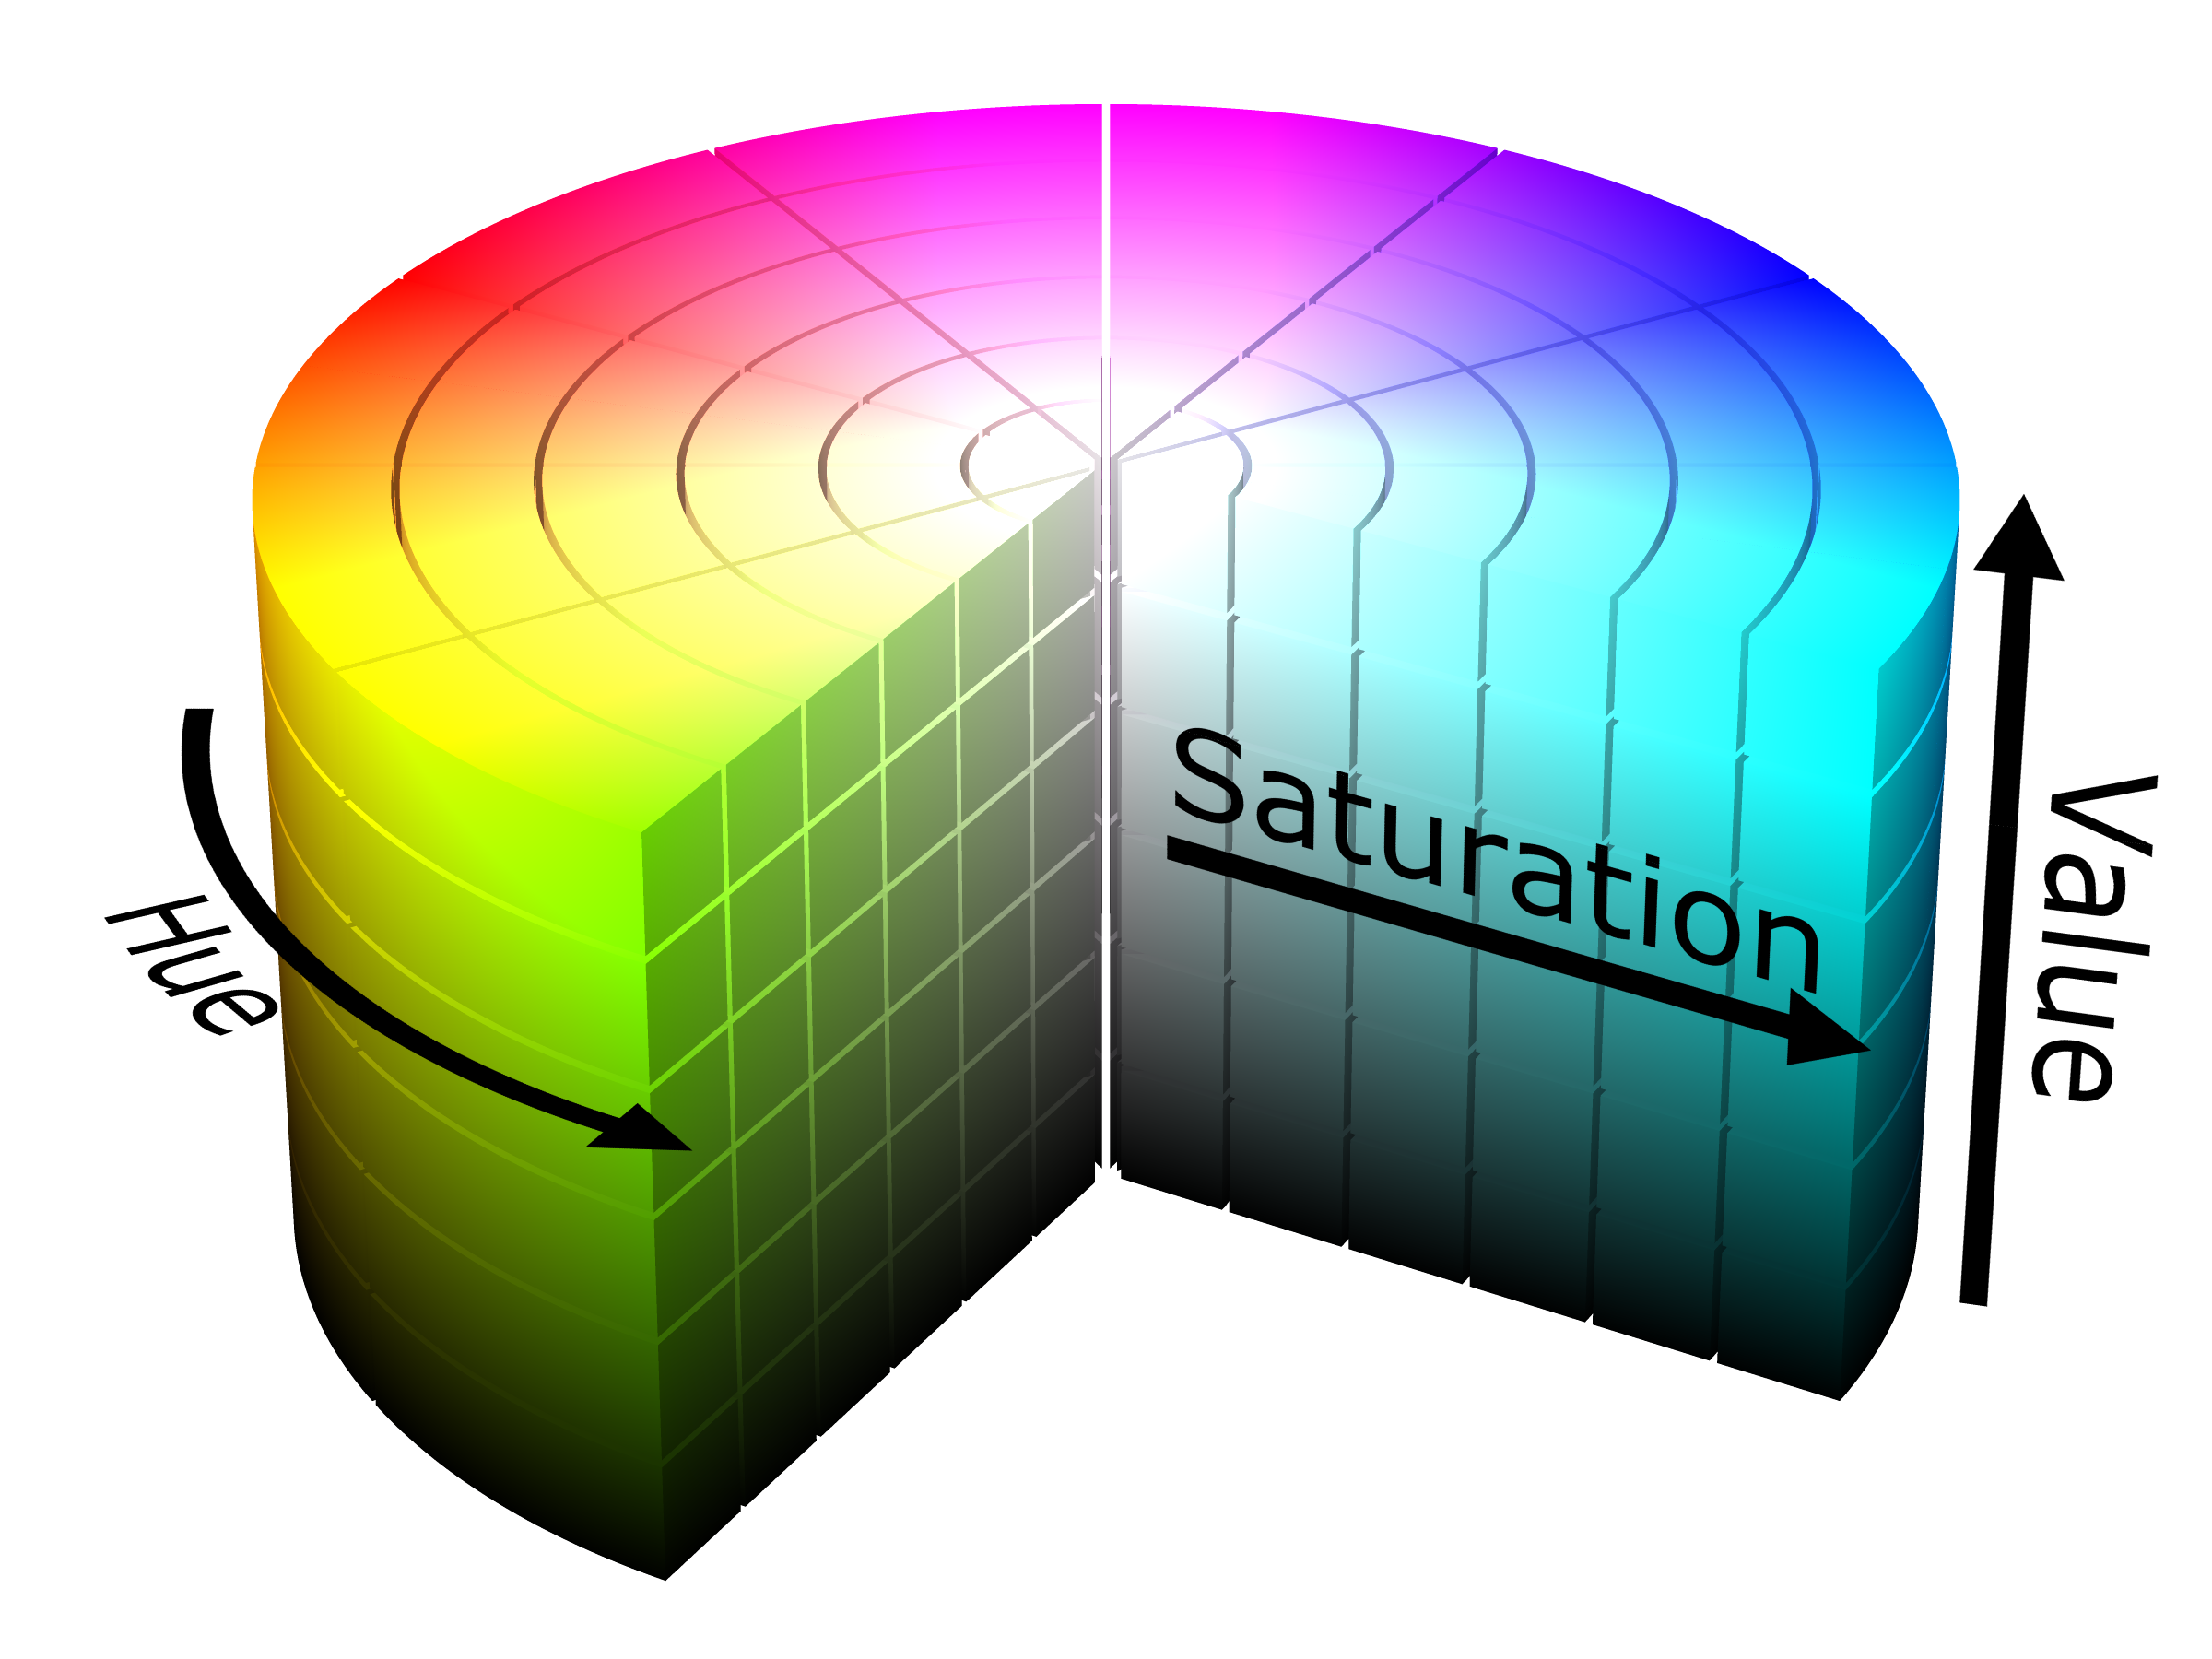
\includegraphics[width=0.65\textwidth]{img/hsv-cylinder.png}
\caption{"HSV cylinder" by SharkD is licensed under CC BY 3.0}
\end{figure}

We describe our algorithm in a few steps. Firstly, we convert our template
image (bounding box) from RGB color space to HSV. Then we choose an average
color in the template. Since the coding of Hue part is placed in the circle, it
is not enough to take a commonly used average. It would cause that image full
of Warm Red (the hue value of this color is circa equal to 15) and Cool Red
(the hue is circa 345) would average to Mid Cyan (hue: 180), instead of Red
(hue 0).

To get a more reasonable average, we take the hue value of each pixel as an
angle. Then we compute the average of the angles. We represent each angle as a
corresponding unit vector from the origin. We sum these vector and get a vector
$(x, y)$. We find a corresponding angle for this vector using $arctang2$
function.  The following formulas describe the process of getting an average
angle.

$$
\begin{aligned}
x &= \sum_\alpha cos \alpha \\
y &= \sum_\alpha sin \alpha \\
\alpha_{avg} &= arctang2(y, x)
\end{aligned}
$$

The use of this algorithm for one colored object is displayed in the figure
\ref{fig:hsv-tracker}. We consider as a disadvantage that no other objects of
the same color can be placed in the view of the camera.

\begin{figure}
  \centering
  \begin{subfigure}[b]{0.48\linewidth}
    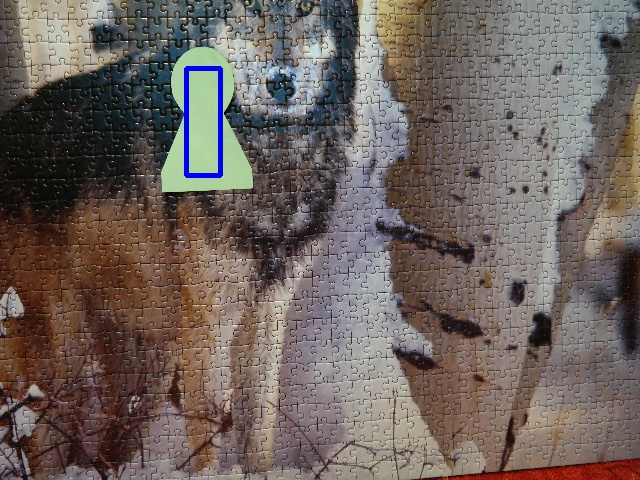
\includegraphics[width=\linewidth]{img/hsv/initial.jpg}
    \caption{Initial image with selected object}
  \end{subfigure}
  \begin{subfigure}[b]{0.48\linewidth}
    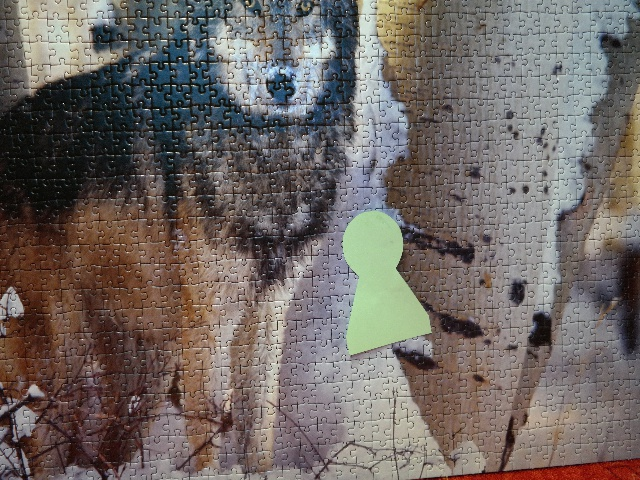
\includegraphics[width=\linewidth]{img/hsv/object.jpg}
    \caption{Image with moved object}
  \end{subfigure}
  \begin{subfigure}[b]{0.48\linewidth}
    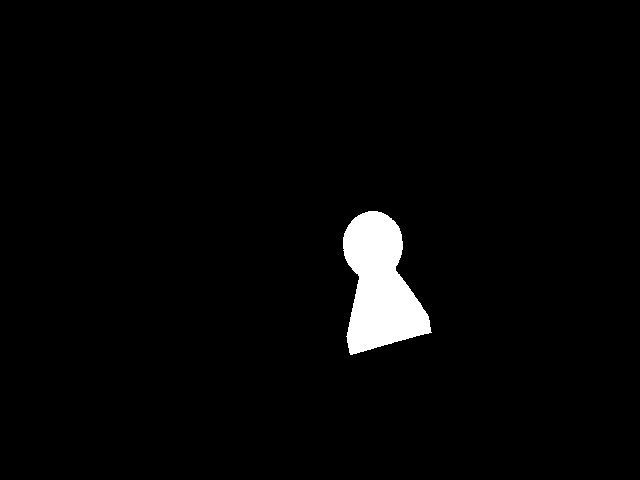
\includegraphics[width=\linewidth]{img/hsv/mask.jpg}
    \caption{Mask created by looking for similar colors}
  \end{subfigure}
  \begin{subfigure}[b]{0.48\linewidth}
    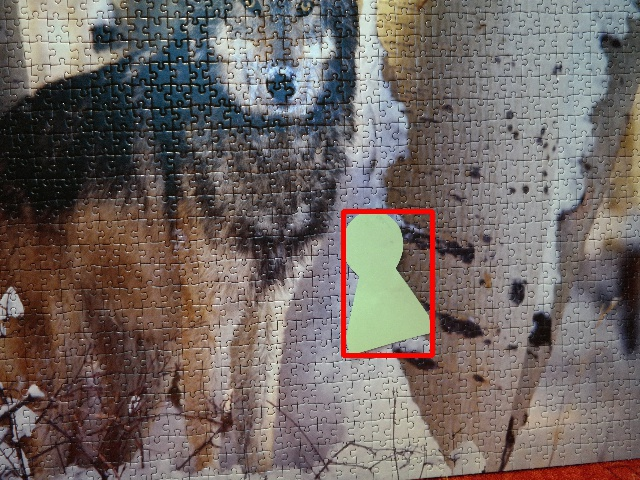
\includegraphics[width=\linewidth]{img/hsv/result.jpg}
    \caption{Bounding box of the largest contour found.}
  \end{subfigure}
  \caption{Process of the HSV tracker}
  \label{fig:hsv-tracker}
\end{figure}

\subsection {Pattern matching}
Pattern (or template) matching algorithm slides over the input image and
compare the template with the patch of the input image.

For patch and template comparison many different metrics may be used. We use
square distance.

Metric could be written as:
$$
R(x, y) =
%\frac{
\sum_{x', y'} (T(x', y') - I(x + x', y + y'))^2
%}{
%\sqrt{\sum_{x', y'} T(x', y')^2 \cdot \sum_{x', y'} I(x+x', y+y')^2}
%}
$$
where $x'$ and $y'$ denotes points from the neighbourhood of the $x, y$. $T$
denotes our pattern and $I$ denotes a patch from the input image. It simply
sums squared distance between corresponding pixels in the pattern and the
patch. From the computed value for each pixel the one with the lowest value
(i.e. shortest distance) is our estimation of the position of the object.

This algorithm works only on grayscale images. Since then much information is
lost during conversion. This disadvantage summed up with no ability to
recognize rotated or slightly changed objects results in unsatisfying tracking
results. A process of correct match and also incorrect one is displayed in the
figure
\ref{fig:pattern-matching-tracker}.

\begin{figure}
  \centering
  \begin{subfigure}{0.48\linewidth}
    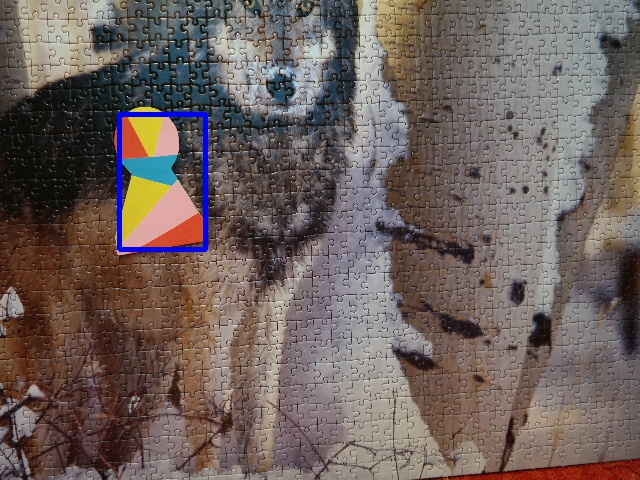
\includegraphics[width=\linewidth]{img/pattern_matching/initial.jpg}
    \caption{Initial image with selected object}
  \end{subfigure}
  \begin{subfigure}{0.48\linewidth}
    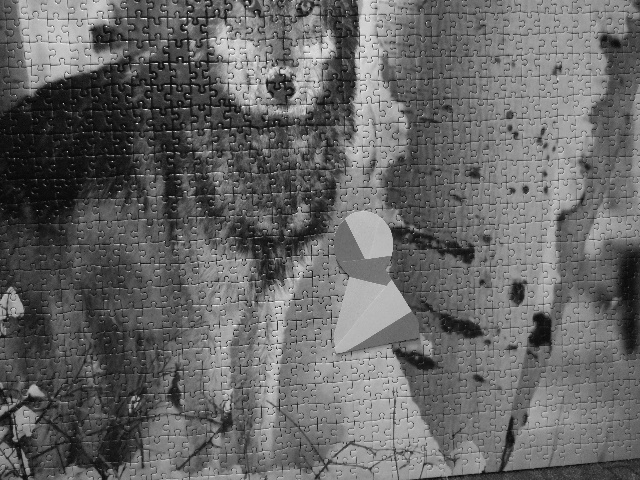
\includegraphics[width=\linewidth]{img/pattern_matching/blackwhite.jpg}
    \caption{Converting it to black white}
  \end{subfigure}
  \begin{subfigure}{0.48\linewidth}
    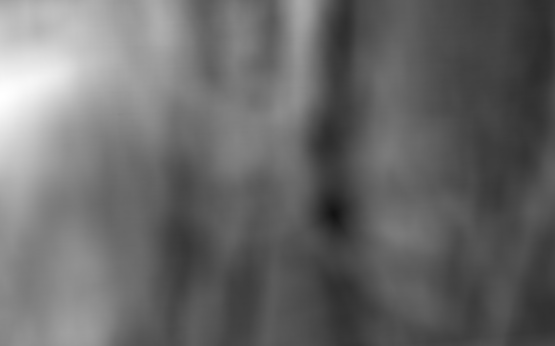
\includegraphics[width=\linewidth]{img/pattern_matching/mask.jpg}
    \caption{Mask created by applying metric}
  \end{subfigure}
  \begin{subfigure}{0.48\linewidth}
    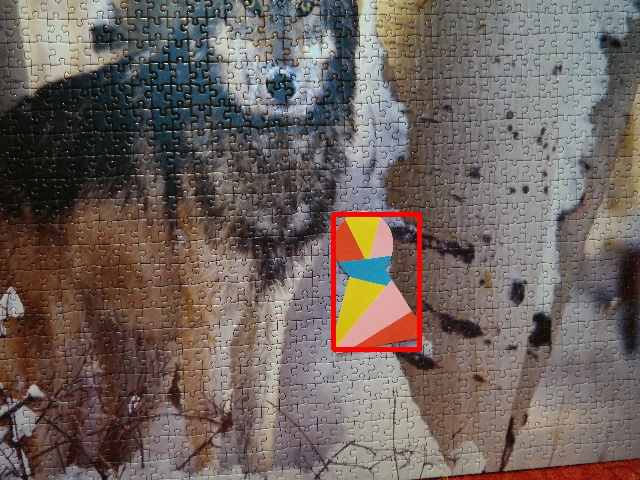
\includegraphics[width=\linewidth]{img/pattern_matching/result-correct.jpg}
    \caption{Darkest point (lowest value) from mask is choosed}
  \end{subfigure}
  \begin{subfigure}{0.48\linewidth}
    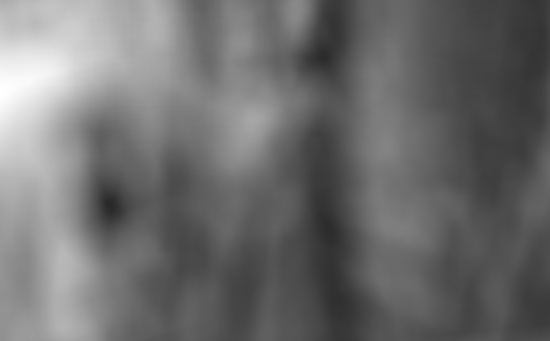
\includegraphics[width=\linewidth]{img/pattern_matching/mask-incorrect.jpg}
    \caption{Mask with darkest point on the left}
  \end{subfigure}
  \begin{subfigure}{0.48\linewidth}
    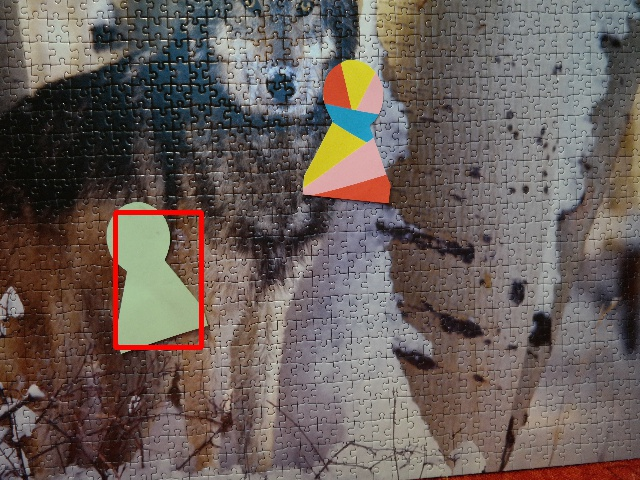
\includegraphics[width=\linewidth]{img/pattern_matching/result-incorrect.jpg}
    \caption{Incorrectly matched pattern}
  \end{subfigure}
  \caption{Process of the pattern matching}
  \label{fig:pattern-matching-tracker}
\end{figure}


%%%%%%%%%%%%%%%%%%%%%%%%%%%%%%%%%%%%%%%%%%%%%

\section{Sequence-based algorithms}

We denote as sequence-based algorithms a class of tracking algorithms, which
are using information from several previous and current image to track.

Using the advantage of information from previous frames could create not only
more stable but also faster trackers. Tracking preserves identity, which means
that also in the case of multiple moving objects it remains to track the original
one.

Samples of the information we can obtain from sequence of the images:
\begin{itemize}
\item velocity -- from previous images we can estimate speed and the direction of
  the movement. This information can reduce the searching area to smaller one
  and increase the speed of the algorithm.
\item appearance -- object may rotate and change its shape or color. Tracker able to
  learn can be persistable against such changes
\end{itemize}

An algorithm using this information can cope with occlusion - what usually
detection algorithms are not able.

In the next sections, we will present few trackers implemented in the OpenCV. We
provide a short overview of the trackers available.

\subsection*{BOOSTING tracker}
Boosting tracker is based on online AdaBoost. It considers bounding box as
positive sample and patches of background as negative ones. For a new image, a
classifier runs on every pixel in the neighborhood of the previous location,
scoring every pixel. The location with the highest score is chosen as a new
location. The implementation in OpenCV is based on \citet*{boosting}.

\subsection*{MIL tracker}
The MIL is a shortcut for Multiple Instance Learning. In comparison to the
BOOSTING tracker, it does not keep only one image of positive example, but the
whole bunch of the images. Tracker considers a small neighborhood of the
current position as possible positive examples. It helps tracker to cope with
the occlusion. OpenCV implementation is based on \citet*{mil}.

\subsection*{KCF tracker}
KCF stands for Kernelized Correlation Filters. Similarly, as the MIL tracker,
it uses more positive samples and their large overlapping regions.
Implementation provided by OpenCV is based on \citet*{kcf}.

\subsection*{TLD tracker}
Tracking, learning and detection, these are the three components of this
tracker. The tracker works frame to frame, and detection corrects the tracker
if necessary. The learning estimates detector's errors and updates it to avoid
these errors in the future. The implementation in OpenCV is based on \citet*{tld}.

\subsection*{MEDIANFLOW tracker}
This tracker focus on forward-backward error trying to minimize it. The
implementation in OpenCV is based on \citet*{medianflow}.

\subsection*{MOSSE tracker}
MOSSE tracker is proposed for fast object tracking using correlation filter
methods. Firstly it does Fast Fourier Transform for template and the image.
Then an convolution operation is performed between the images and the result is
inverted by Inverse Fast Fourier Transform (IFFT). The position is estimated by
the highest value of the IFFT response. More about the tracker is available in
the paper by \citet*{mosse}.

\subsection*{OpenCV note}
OpenCV-contribute implements all these sequence-based trackers GOTURN tracker
is also implemented in OpenCV. Unfortunately, at the time of the writing
thesis, it contains bug causing it unusable. An overview of OpenCV trackers is
provided by \citet*{opencv-trackers}.

\subsection*{Correlation tracker}
For a comparison we decided to include a tracker implemented in Dlib. This correlation tracker is based on the paper by \citet*{correlation}.

%%%%%%%%%%%%%%%%%%%%%%%%%%%%%%%%%%%%%%%%%%%%%

%\section{Comparison of trackers}
%
%\subsubsection{Experiment with simplyfied environment}
%
%Given a video sequence XYZ second long we studied an accuracy of trackers. The background is one colored and moving object is a red circle.
%
%\todo[inline]{ Robot sledujúci čiaru do štvorca s červeným kruhom z vrchu (kamery sa dívajú zvrchu). Porovnanie bude uvedené ako čiary, ktoré sú nakreslené pomocou zachytených bodov.}
%
%\subsubsection{Experiment in complex environment}
%
%Background consisted of many colors and patterns. Moving object has a pattern and is partially colored as the background.
%
%\todo[inline]{ Vyskytli sa veci, ako, že stratil polohu? V akom percente? Mám ako rozumne vyjadriť presnosť tých súradníc lepšie než od oka?}
